
\section{Introduction}
Biological species are well recognized as being engaged in an evolutionary fight-for-survival and Game Theory has been used to analyze the strategies in such a fight.
This analysis is the defining feature of Evolutionary Game Theory, whose many features and concepts are often credited to John Maynard Smith and George R. Price \cite{maynard,maynard2}.
Evolutionary Games can have different forms but one of the most standard evolutionary game-forms concerns the continuous growth/decay of organism types; the organism types are defined by the strategy they play as they are continuously randomly paired to participate in a simultaneous symmetric two-player game where the expected payoff determines each participant's growth.\cite{weibull}

Evolutionary game theory has been a valuable tool in characterizing the dynamics and interactions among biological species and it also has proven utility in other fields which feature evolutionary dynamics.  Some examples of phenomena which have been modeled via Evolutionary Game Theory include: altruism, empathy, human culture, moral behavior, private property, proto-linguistic behavior, social learning, societal norms, personality and mating-dynamics \cite{sep-game-evolutionary,socialpsyc1,Hodgson2012,McNamara953}.

However many organisms exhibit behaviors which are coupled with the state that they are in, and this interaction is not often modeled using the most standard evolutionary game theory.
Some canonical examples include the behavior of perspiring with increasing body temperature causing dehydration, foraging behavior with hunger signals causing food shortage, sleep with ambient light levels causing vulnerability to predation, or hibernation with the change of season causing hunger.

Within this paper we will discuss the nature of 'state' and develop a evolutionary game for modeling this dynamic. We also discuss a notion of equilibrium in the context of the game and give an algorithm which solves for the game's equilibria. We give an example of the game as an extension of the classic Hawk-Dove game\cite{maynard} and we also briefly compare how our game's dynamics compares with the games of others.

\subsection{Motivation}
A concept that is sometimes referred-to in the computer modeling of evolution is of `digital organisms', defined as interacting computer programs designed to test or verify hypotheses about evolution.\cite{Lenski1999, Lenski2003, 10.1371/journal.pbio.0000018} These computer programs may feature a range of different qualities such as simulated position, communication, movement, competition and sexual reproduction and can be self-replicating and/or mutating in-memory. There exist well-developed software platforms to simulate the evolving populations these digital organisms (such as Avida and Darwinbots\footnote{which is a personal favorite of the author} or historically Tierra \cite{ray-approach-to-synthesis-1991}). The use of digital organisms as an avenue of exploring the dynamics of life is associated with the field named 'artificial life' or sometimes abbreviated as 'A-Life' \cite{journals/alife/BedauMPRAGIKR00}\cite{alife1}

Within the configuration of these software platforms the parameters of the simulation are specified. These parameters can be grouped as follows:

\begin{itemize}[leftmargin=*,labelsep=4mm]
\item   The potential \textbf{States} that the organisms can be in, such as their position on a grid or graph, internal conditions such as body temperature, the states of their sensory inputs such as heat or light, their social relationships such as being single or conjoined, as well as the potential states of their own memory.
\item   The \textbf{Actions} which the organisms can execute, such as 'reproduce', 'move', 'eat' and 'sleep'. These actions may only be available to some states and not others, for instance, as an organism may not be able to execute action 'eat' when it is in a state of being 'full', or 'sleep' when in a state 'in daylight'.
\item   The \textbf{Code} or \textbf{Strategy} is private to each organism in the simulation, and simply determines what action/s the organism does depending on the state it is in.
\item   And the \textbf{Consequences} of the actions of the organisms. This can be as simple as a transition between state, for instance the action 'move-left' might change the state executing organism to 'position -1'. And this may be contingent on the state and actions of the other organisms, as 'move-left' might only succeed if there is not another organism in 'position -1' doing action 'move-right'. Alternately actions such as 'reproduce' may add or remove organisms from the simulation entirely and also add random changes into the code of the organisms.
\end{itemize}

As these simulations progress it is possible to analyze the changes in the population and the code of the evolving organisms. Indeed it is possible to watch time-lapse videos of swarms of these digital organisms undergo the evolution of interesting behaviors \textit{in silico}.

Unfortunately the results of these simulations are seldom very deterministic and a badly tuned simulation can easily be devoid of any interesting results. However recent work has been conducted to incorporate some of this potentially complex state-action dynamics into the mathematical framework of evolutionary game theory. It is the objective of the paper to attempt to extend it yet still.

\subsection{Related Work}\label{sec:-1}

A relatively simple example of in which state can be seen in the literature of game theory is in the context of the famous Iterated Prisoners Dilemma. In the Iterated Prisoners Dilemma successful strategies such as 'tit-for-tat', make the player's choice of action a direct function of the memory of previous interactions. It is possible to conceive of the tit-for-tat program (as it existed in the computer cores of Axelrod's famous tournaments \cite{spacial4}) as a particularly simple digital organism.
The organism of tit-for-tat might be modeled as having had a single binary state (storing the opponents previous play) which determined what action would be executed (cooperate or defect) and together with the executed action of the opponent, have determined the consequences - immediate payoffs and state transitions.

Another line of literature in which state can be seen is in the discussion of Markov-Decision-Processes (MDPs). In MDPs there is a single player which has a set of possible states and a set of actions. The strategy (or 'policy') determines what actions the player will execute as a function of what state it is in. The actions that are executed result in probable transitions between the states of the player, and also determine the player's immediate payoffs (or 'rewards').

MDPs bear a strong conceptual similarity with Lloyd Shapley's multiple-player Stochastic-Games (SG) \cite{shapley53}\cite{Solan2015} in which the game itself has a set of possible states or 'positions'. Within this context each of the finite number of players have actions which they can execute. The actions which the players execute determine the transitions between the states of the game and also the immediate payoffs to each of them.

It important to note that in these games the strategies of the participants are evaluated by the expected summations of the payoffs.

Another example in which state can be seen in literature is in the structures of `Spatial Evolutionary Games' and more generally `Evolutionary games on graphs' where the organisms have the state of belonging to nodes on a grid or graph structure. In these games the organisms at a node play actions against their nearest neighbors and/or themself and there is specified a `who-plays-with-who' in the game structure. It can be seen that these games capture a general sense of location as a state for the organisms, and also introduces unique and dynamic behavior.\cite{spacial1,nowak,spacial2,spacial3}
In the structure of these games it is seen that the organisms at the nodes have strategy which determines what action they execute (such as cooperate or defect). And in some of these games the success of a strategy is evaluated by the expected payoff of that the action receives against a weighted combination of the organism's neighbors.

Specifically we note that in Szabó and Fáth\cite{spacial4} there is faithfully detailed a large collection of these games and the reader is encouraged to compare the structure of our game with them.

Another approach of integrating state into game theory extends from the pioneering work of Eitan Altman, and his colleagues Ilaria Brunetti and Yezekael Hayel \cite{markov2,markov3,markov4,markov5,markov8,markov9} who introduce the Markov-Decision-Evolutionary-Game (MDEG) and variants thereof.

In MDEG games each organism can occupy one of a finite set of states, and has actions available to it depending on what state it is in.
Within the population, the organisms are paired randomly and each of the participants chooses one of their available actions (as determined by their strategy) to execute.
Within this interaction the actions that the two organisms execute determine the immediate payoff to both and also the probable transitions in state that the organisms will make.
In these games the expected long-term expected sum of payoffs that the organisms receives for their strategy determine the growth-rate of the presence of the strategy in the population.
This growth then changes the composition of the population in which the pairings occur.

Several example MDEG games are introduced in Altman's literature including modifications and extensions of the most classic Hawk-Dove game, from which we take inspiration.\cite{markov3,markov5}
MDEG includes many features for modeling state-action interactions within evolutionary game theory and serves to provide a primary contrast for our game.

Within MDEG games, the transitions between states bear close similarity with markov transitions between state (such as embedded in MDPs), and we hope to show in this paper that by relaxing this markov property we get a game that is quite different and hopefully more powerful in its potential for representing evolutionary phenomena.

Before truly beginning the body of the document, it is worth stating that we will sometimes make cartoon illustrations.
This is done in an attempt to soften the presentation of mathematical content, to highlight core concepts and to encourage the imagination of the reader - it is not intended to be belittling or making light of any content or concepts whatsoever.

\subsection{Structure}
The remainder of this paper is organised as follows: section \ref{sec:2} presents the core concept of non-markovian transmission of organisms between states, section \ref{section:formalism} gives formalism to the non-markovian game and its algorithm, section \ref{sec:equilibria} discusses the game's equilibria and gives confinement for the algorithm's equilibria search, section \ref{sec:example} details a Hawk-Dove game as example of the working algorithm, and section \ref{sec:discussion} concludes the paper with some general comments about the features and limits of our game.

\section{Non-Markov transmission}\label{sec:2}

Suppose for a moment that we wanted to make an evolutionary model of the behavior of an organism, such as a monkey.
We might describe the monkey as having states and actions, such as 'being in a tree' or 'throwing a banana'.
And these actions might have consequences on the state of the monkey and perhaps of other monkeys in our population.
All of this can be described by existent models in literature, some of which are described in section \ref{sec:-1}.

There is a question that motivates the model and content of this paper, it is:\\ \textit{"What do the payoff values mean?"}\\
Suppose that our hypothetical monkey 'in a tree' did action 'throw banana' at an opponent and received an immediate payoff of -1.7.  What could this correspond to?\\
If the value were very positive we might think of it as relating to how many offspring the monkey might be likely to have, or if very negative then relating to the monkeys death.
Indeed it is seen that in some Evolutionary Games the relative 'success' or 'fitness' of a particular strategy is related to the sum of these values.\\
It is also worth noting that fitness is not a very simple concept\cite{sep-fitness}. We might think of a strategy as being fitter if the organism using it is more functional in its environment (conceived statically) and/or fitter if it assists the survival of the genes of its family. But if the family members are also competitors for resources then relative fitness might not be particularly easy to determine - especially if many other factors are considered and included.

In any-case, the primary drive of this paper is to attempt a game-theoretic model of evolution that bypasses these questions.\\
At no point in our model do we specify the payoffs for actions. For instance, if a payoff of +2 is to be interpreted as 'having two offspring' we attempt to have the model facilitate that outcome directly - by actually generating two additional monkeys perhaps in state 'healthy baby' - who might then proceed to do action 'feed' which then might change daddy monkey's 'resource level' state and etc.

In order to model this effect at a population-level it is unfortunate that some of the details of between the organisms would have to be lost - such as the detail about which baby monkeys belong to what daddy. Such individual relationships would seem difficult to model without considering the particular organisms on an individual level.\footnote{Although there is nothing blocking a population-level consideration of having monkey organisms changing from a state of 'daddy having 1 baby' to 'daddy having 2 babies', and at the same time have monkeys changing from state 'baby having no siblings' to state 'baby with one sibling', for instance.}

Instead what can be modeled is the total number of the organisms in each of the potential states, and consider that the organisms that execute a particular action such as 'reproduce' might increase the total number of organisms in other states.
Another instance of an action that is seen to affect the total number of organisms between states is movement. If an individual monkey executes action 'moves north' it could be seen to decrease the number of organisms in its original state and increase it in another. In this context the monkey is generally said to 'transition' between the two states.
In these examples of reproduction and movement there can be seen to be demographic flow from one state into others.
And since it seems odd to say that a daddy monkey 'transitions' into baby monkeys we use the term \textit{transmission} to capture the broader notion.\footnote{As might be said that: "the daddy monkey \textit{transmits} its kind into the baby state"; the emphasis of the sentence is to flag the reader to the subtle difference in the spelling.}

The demographic flow of individuals of a species' population between states is sometimes described in ecological-studies by a matrix that is not necessarily markov.\cite{population1}
The simplest example of such matrices are Leslie Matrices used for studying the structure of populations of individuals transitioning between evenly spaced age-states.
Leslie Matrices are square, and they have form \cite{leslie}:

\begin{equation*}
M=\begin{bmatrix}
    F_0 & F_1 & F_2 & \dots  & F_{m-2} & F_{m-1} & F_m  \\
    P_0 &  0  &  0  & \dots  &    0    &  0      &  0   \\
     0  & P_1 &  0  & \dots  &    0    &  0      &  0   \\
     0  &  0  & P_2 & \dots  &    0    &  0      &  0   \\
    \vdots & \vdots & \vdots & \ddots & \vdots & \vdots & \vdots \\
     0  &  0  &  0  & \dots  & P_{m-2} &  0      &  0   \\
     0  &  0  &  0  & \dots  &    0    & P_{m-1} &  0   \\
\end{bmatrix}
~~~0<P_x<1;~~F_x\ge0
\end{equation*}
Where $P_i$ represents the probability of and individual in the $i$th age bracket successfully living into the $(i+1)$th age bracket, and $F_i$ is average number of offspring for an individual in $i$th age bracket within the duration of the age bracket.
For a column vector $n = [n_0,n_1,n_2,\dots,n_m]$ with each $n_i$ representing the number of individuals in each age-bracket, $Mn$ gives the expected number of individuals in the population after the duration of one age bracket of time, and $M^2n$ the expectation individuals after two age brackets, $M^3n$ after three, and so on.
Successive applications eventually yield a steady population profile between the $n_i$, and a constant exponential growth rate $\lambda$ given by the Euler–Lotka equation.
The $\lambda$ is the dominant and only real-positive eigenvalue of the matrix, with the steady distribution $n$ as its corresponding eigenvector, that is $Mn=\lambda n$.

Although the elements in the Leslie matrix are positive and represent the states of organisms in the population and the transition between, the matrix isn't Markov because its columns (or alternatively rows) don't necessarily sum to one.  The informal difference is that whereas in a Markov-chain matrix the elements represent the expectation of \textit{transition} between states, Leslie matrix elements represent the expectation of \textit{transmission} between states inclusive of such possible factors as births and deaths.
We term the class of such matrices as `transmission matrices' in this article and assert the only thing defining such matrices are that they are real, square and have non-negative elements.\footnote{General non-negative real square matrices (or at-least irreducible ones) have at-least one real non-negative eigenvalue (via indirect application of Perron-Frobenius theorem, see chapter 3 of \cite{matrix2}) hence a transmission matrix identifies at-least one growth-rate}
We do this because such matrices can be built more broadly than simple Leslie-matrix form\cite{models1,models2}. Consider the rich interaction between organism-states captured by the matrix of transmissions for the 'Nodding Thistle' in figure \ref{fig:1}.



\begin{figure}[h]
    \begin{subfigure}[b]{.5\linewidth}
        \centering
        \begin{tikzpicture}[scale=0.9, transform shape,->,>=stealth',shorten >=1pt,auto,node distance=1.7cm,thick,main node/.style={circle}]
            \path[use as bounding box] (-2.5cm, -2.8cm) rectangle (2.5cm, 2.5cm);
            \node[main node] (SB)  at (-2cm,  2cm) [align=center, text width=2.1cm] {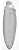
\includegraphics[width=.05\textwidth]{1.png}\\\small Seed};
            \node[main node] (SM)  at ( 2cm,  2cm) [align=center, text width=2.1cm] {
\includegraphics[width=.25\textwidth]{2.png}\\\small Small};
            \node[main node] (ME)  at ( 2cm, -2cm) [align=center, text width=2.1cm] {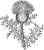
\includegraphics[width=.29\textwidth]{3.png}\\\small Medium};
            \node[main node] (LE)  at (-2cm, -2cm) [align=center, text width=2.1cm] {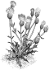
\includegraphics[width=.38\textwidth]{4.png}\\\small Large};

            \node[main node] (SBm) at (-2cm,  2cm) [align=center, text width=1.2cm] {};
            \node[main node] (SMm) at ( 2cm,  2cm) [align=center, text width=1.2cm] {};
            \node[main node] (MEm) at ( 2cm, -2cm) [align=center, text width=1.2cm] {};
            \node[main node] (LEm) at (-2cm, -2cm) [align=center, text width=1.2cm] {};

            \path[every node/.style={sloped,auto=false}]
            (SBm) edge [in=180-20,out=180+20,looseness=3,   line width=1pt,anchor=south] node  {\scriptsize 0.443} (SBm)
            (SBm) edge [bend left=15,                       line width=1pt,anchor=south] node  {\scriptsize 0.0039} (SMm)
            (SBm) edge [bend left=15,                       line width=1pt,anchor=south] node  {\scriptsize 0.0004} (MEm)
            (SBm) edge [bend left=15,                       line width=1pt,anchor=south] node  {\scriptsize 0.0005} (LEm)

            (SMm) edge [bend left=15,                       line width=1pt,anchor=south] node  {\scriptsize 0.1584} (SBm)
            (SMm) edge [in=20,out=-20,looseness=3,          line width=1pt,anchor=north] node  {\scriptsize 0.0078} (SMm)
            (SMm) edge [bend left=15,                       line width=1pt,anchor=south] node  {\scriptsize 0.0031} (MEm)
            (SMm) edge [bend left=15,                       line width=1pt,anchor=north] node  {\scriptsize 0.01} (LEm)

            (MEm) edge [bend left=15,                       line width=1pt,anchor=north] node  {\scriptsize 6.6105} (SBm)
            (MEm) edge [bend left=15,                       line width=1pt,anchor=south] node  {\scriptsize 0.2434} (SMm)
            (MEm) edge [in=-20,out=20,looseness=3,          line width=1pt,anchor=south] node  {\scriptsize 0.0314} (MEm)
            (MEm) edge [bend left=15,                       line width=1pt,anchor=south] node  {\scriptsize 0.0613} (LEm)

            (LEm) edge [bend left=15,                       line width=1pt,anchor=south] node  {\scriptsize 206.56} (SBm)
            (LEm) edge [bend left=15,                       line width=1pt,anchor=south] node  {\scriptsize 7.6091} (SMm)
            (LEm) edge [bend left=15,                       line width=1pt,anchor=south] node  {\scriptsize 0.793} (MEm)
            (LEm) edge [in=180+20,out=180-20,looseness=3,   line width=1pt,anchor=north] node  {\scriptsize 0.945} (LEm)
            ;
        \end{tikzpicture}

        \caption{Life cycle graph of the population model}\label{fig:1a}
    \end{subfigure}
    \begin{subfigure}[b]{.5\linewidth}
        \centering
        \footnotesize
        $$ \begin{bmatrix}\text{Seed}_{t+1}\\\text{Small}_{t+1}\\\text{Medium}_{t+1}\\\text{Large}_{t+1}\end{bmatrix}= 
        \begin{bmatrix}
            0.443&0.1584&6.6105&206.56\\
            0.039&0.0078&0.2434&7.6091\\
            0.0004&0.0031&0.0314&0.793\\
            0.0005&0.01&0.0613&0.945
        \end{bmatrix}
        \begin{bmatrix}\text{Seed}_{t}\\\text{Small}_{t}\\\text{Medium}_{t}\\\text{Large}_{t}\end{bmatrix}$$
        \caption{
            4x4 matrix model of a Nodding Thistle (\textit{Carduus nutans}) population in Australia, classification based on seed - and rosette size. The transmission numbers represent aggregate survival/growth/propagation of individuals from one class into another per year. The projected population growth rate ($\lambda$) is 1.207 per year.\\
      Data from Jongejans et.al\cite{models2}\\ Original data from Shea et.al\cite{models3}
        }\label{fig:1b}
    \end{subfigure}
        \vspace{-2.3\baselineskip}
    \caption{}\label{fig:1}
\end{figure}

We might imagine that if we had a cohort of 100 monkeys in a state 'with banana' whose strategy dictated that they do action 'throw banana' that this might result in 75 monkeys moving to a state 'without banana' and 25 remaining in state 'with banana'. In this case the monkeys of this certain strategy might be described by such a matrix with 0.75 and 0.25 as elements.
We might imagine that a cohort of 100 monkeys in a state 'south' did action 'attempt migrate north' might result in 120 monkeys in state 'north' and 20 monkeys remaining in state 'south'. In this case the monkeys of the strategy might be described by a matrix with 1.2 and 0.2 as elements.

It is by these transmission matrices that we are able to highlight the notion of transmission between two states as being the demographic flow of the population from one to the other.
This notion forms a core concept in the next section as we formalize states and actions for the organisms and thence proceed to compare strategies in game-theory analysis for equilibria.

